Para realizar o experimento foram gerados 100 pontos válidos para cada mapa, e então selecionados os valores que eram válidos nos 3 mapas.

\subsection{Custo total}
Os pontos avaliados são mostrados nas tabela~\ref{tab:total-costs-1},~\ref{tab:total-costs-2} e~\ref{tab:total-costs-3}. É possível observar que o custo dos algoritmos A* com \textit{distância octile}, UCS e IDS são iguais, uma vez que esses algoritmos são ótimos. Já o custo do algoritmo guloso é, na maioria das vezes, maior do que o ótimo. Isso se deve a sua natureza gulosa, que busca encontrar o primeiro resultado possível, sem se preocupar com o resultado ótimo. Em alguns casos, pode haver uma interrupção no meio do caminho, que o algoritmo guloso não leva em conta previamente, resultando em um caminho total de custo maior.

\begin{table}[htbp]
\centering
\caption{Custo total para o mapa 1}
\label{tab:total-costs-1}
\begin{tabular}{ll|lllll}
\multicolumn{2}{c|}{Points}  & \multicolumn{5}{c}{Total Cost} \\ \hline
Initial & Final & A* Octile & A* Manhattan & BG    & UCS   & IDS   \\ \hline
167,173       & 232,224     & 90.5      & 90.5         & 90.5  & 90.5  & 90.5  \\
92,218        & 184,181     & 110.5     & 110.5        & 111.5 & 110.5 & 110.5 \\
95,165        & 74,69       & 120       & 120          & 124   & 120   & 120   \\
138,133       & 26,160      & 140.5     & 140.5        & 150   & 140.5 & 140.5 \\
193,73        & 246,155     & 214       & 214          & 240   & 214   & 214   \\
174,14        & 53,61       & 241.5     & 241.5        & 293.5 & 241.5 & 241.5 \\
33,218        & 26,98       & 254.5     & 259.5        & 379   & 254.5 & 254.5
\end{tabular}
\end{table}

\begin{table}[htbp]
\centering
\caption{Custo total para o mapa 2}
\label{tab:total-costs-2}
\begin{tabular}{ll|lllll}
\multicolumn{2}{c|}{Points} & \multicolumn{5}{c}{Total Cost}\\ \hline
Initial & Final & A* Octile & A* Manhattan & BG    & UCS   & IDS   \\ \hline
167,173       & 232,224     & 93        & 93           & 94    & 93    & 93    \\
92,218        & 184,181     & 115       & 115.5        & 117   & 115   & 115   \\
95,165        & 74,69       & 214       & 214          & 236   & 214   & 214   \\
138,133       & 26,160      & 365       & 365          & 460.5 & 365   & 365   \\
193,73        & 246,155     & 122.5     & 122.5        & 122.5 & 122.5 & 122.5 \\
174,14        & 53,61       & 154.5     & 154.5        & 238   & 154.5 & 154.5 \\
33,218        & 26,98       & 226.5     & 226.5        & 268.5 & 226.5 & 226.5
\end{tabular}
\end{table}

\begin{table}[htbp]
\centering
\caption{Custo total para o mapa 3}
\label{tab:total-costs-3}
\begin{tabular}{ll|lllll}
\multicolumn{2}{c|}{Points} & \multicolumn{5}{c}{Total Cost}      \\ \hline
Initial & Final & A* Octile & A* Manhattan & BG    & UCS   & IDS  \\ \hline
167,173       & 232,224     & 107       & 107          & 110   & 107   & 107   \\
92,218        & 184,181     & 129       & 129          & 142   & 129   & 129   \\
95,165        & 74,69       & 129.5     & 129.5        & 170   & 129.5 & 129.5 \\
138,133       & 26,160      & 125.5     & 126.5        & 142   & 125.5 & 125.5 \\
193,73        & 246,155     & 171.5     & 171.5        & 174.5 & 171.5 & 171.5 \\
174,14        & 53,61       & 144.5     & 144.5        & 155.5 & 144.5 & 144.5 \\
33,218        & 26,98       & 245       & 245          & 318.5 & 245   & 245  
\end{tabular}
\end{table}

Foram selecionados alguns outros pontos para se comparar melhor as heurísticas para o algoritmo A*, de forma a mostrar que a heurística de \textit{distância Manhattan} não é ótima. Esses pontos são mostrados na tabela~\ref{tab:a-total-costs}. A heurística de \textit{distância octile} é admissível e consistente, portanto a sua utilização torna o algoritmo ótimo. Já a heurística da \textit{distância Manhattan} não é admissível e consistente, de forma que o resultado obtido nem sempre é ótimo, como se pode observar.

\begin{table}[htbp]
\caption{Custos totais para cada heurística do A*}
\label{tab:a-total-costs}
\begin{adjustbox}{max width=\textwidth}
\begin{tabular}{llll|llll|llll}
\multicolumn{4}{c}{Map 1} & \multicolumn{4}{c}{Map 2} & \multicolumn{4}{c}{Map 3} \\ \hline
\multicolumn{2}{c}{Points} & \multicolumn{2}{c}{Total Cost} & \multicolumn{2}{c}{Points} & \multicolumn{2}{c}{Total Cost} & \multicolumn{2}{c}{Points} & \multicolumn{2}{c}{Total Cost} \\ \hline
\multicolumn{1}{c}{Initial} & \multicolumn{1}{c}{Final} & \multicolumn{1}{c}{Manhattan} & \multicolumn{1}{c|}{Octile} & \multicolumn{1}{c}{Initial} & \multicolumn{1}{c}{Final} & \multicolumn{1}{c}{Manhattan} & \multicolumn{1}{c|}{Octile} & \multicolumn{1}{c}{Initial} & \multicolumn{1}{c}{Final} & \multicolumn{1}{c}{Manhattan} & \multicolumn{1}{c}{Octile} \\ \hline
58,112 & 205,70 & 198.0 & 184.0 & 92,218 & 184,181 & 115.5 & 115.0 & 97,165 & 47,236 & 99.5 & 96.5 \\
91,170 & 144,41 & 197.0 & 192.0 & 213,79 & 104,12 & 157.0 & 153.0 & 153,229 & 69,195 & 104.5 & 102.5 \\
163,247 & 215,93 & 225.0 & 217.0 & 251,25 & 92,13 & 166.5 & 166.0 & 58,18 & 149,22 & 105.5 & 104.0 \\
45,70 & 241,106 & 262.5 & 253.0 & 236,125 & 65,162 & 269.0 & 267.5 & 107,145 & 38,205 & 124.0 & 115.5 \\
33,218 & 26,98 & 259.5 & 254.5 & 200,249 & 147,16 & 325.5 & 320.5 & 138,133 & 26,160 & 126.5 & 125.5 \\
212,2 & 69,180 & 262.5 & 259.5 & 225,229 & 32,55 & 325.0 & 322.5 & 212,163 & 135,232 & 146.0 & 145.5 \\
189,12 & 113,184 & 267.5 & 264.5 & 249,134 & 34,130 & 372.5 & 371.0 & 85,17 & 164,127 & 151.0 & 150.0 \\
57,238 & 4,11 & 334.5 & 329.5 & 244,213 & 54,68 & 384.0 & 380.5 & 30,93 & 152,2 & 200.5 & 196.5 
\end{tabular}
\end{adjustbox}
\end{table}


\subsection{Estados expandidos}
O número total de nós expandidos para cada algoritmo é mostrado nas figuras~\ref{fig:expanded1},~\ref{fig:expanded2} e~\ref{fig:expanded3}. Como é possível observar, a quantidade de nós expandidos no algoritmo IDS é muito grande. Isso se deve em parte ao fato de o algoritmo executar por diversas iterações, de forma que algumas expansões são repetidas a cada iteração. Nas iterações em que o limite de profundidade não permite que uma solução seja encontrada, serão expandidos todos os estados dentro do limite.

\begin{figure}[!htb]
\begin{minipage}{0.5\linewidth}
\centering
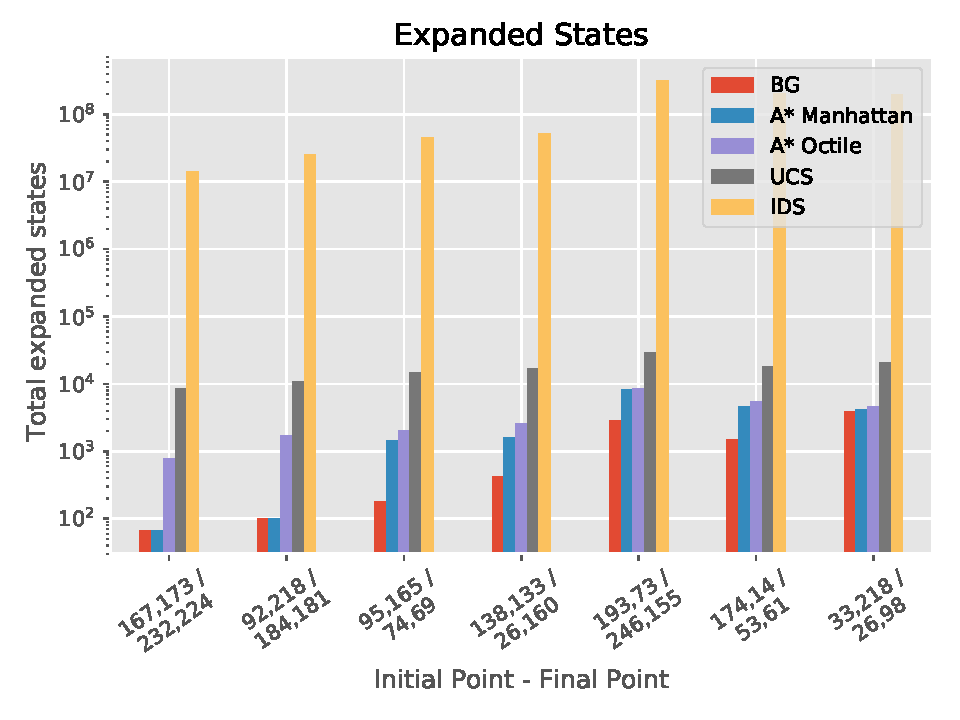
\includegraphics[width=\textwidth]{Images/Expanded_States_map1_log.pdf}
\caption{Estados expandidos para o mapa 1 em escala logarítmica}
\label{fig:expanded1}
\end{minipage}%
\begin{minipage}{0.5\linewidth}
\centering
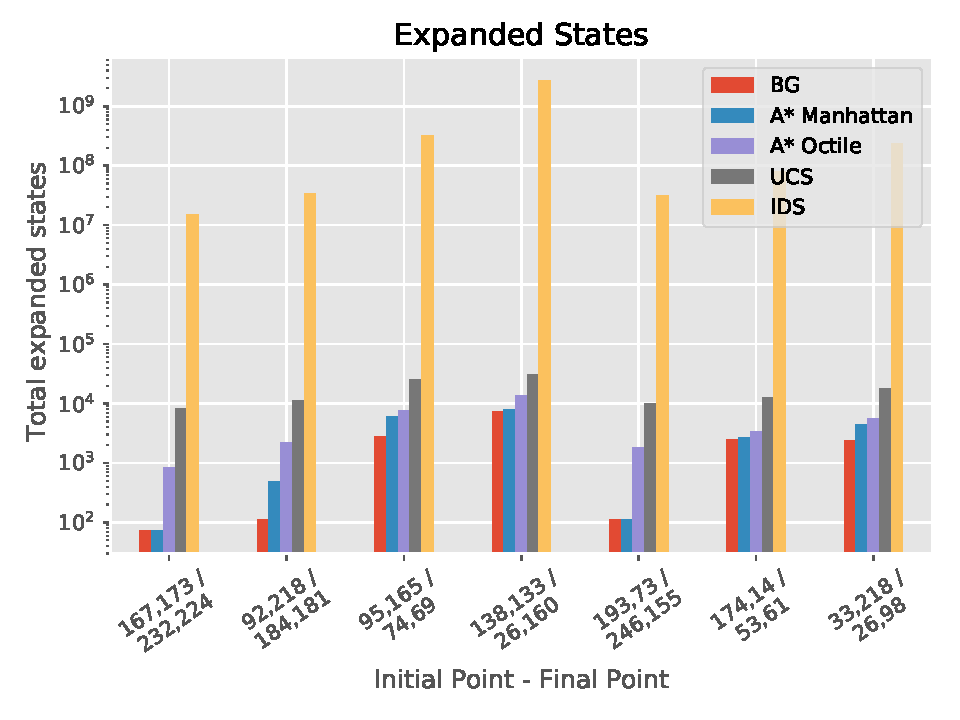
\includegraphics[width=\textwidth]{Images/Expanded_States_map2_log.pdf}
\caption{Estados expandidos para o mapa 2 em escala logarítmica}
\label{fig:expanded2}
\end{minipage}
\begin{minipage}{0.5\linewidth}
\centering
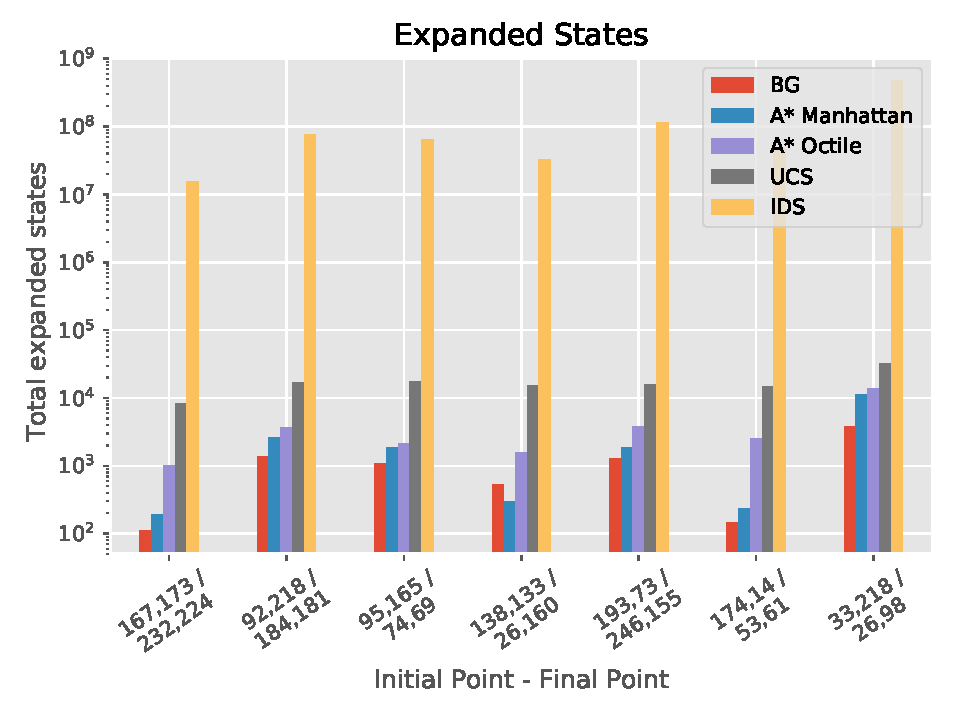
\includegraphics[width=\textwidth]{Images/Expanded_States_map3_log.pdf}
\caption{Estados expandidos para o mapa 3 em escala logarítmica}
\label{fig:expanded3}
\end{minipage}
\end{figure}

O algoritmo de \textit{Best first Search} expande o menor número de estados, devido à sua caraterística gulosa. Isso faz com que o algoritmo muitas vezes não expanda os estados pertencentes à solução ótima. O UCS, expande um número grande de estados comparado com os algoritmos A*, por não ser uma busca com informação. Dessa forma ele precisa buscar muito mais estados pelo objetivo, enquanto o A* possui um certo direcionamento.

\begin{figure}[!htb]
\begin{minipage}{0.5\linewidth}
\centering
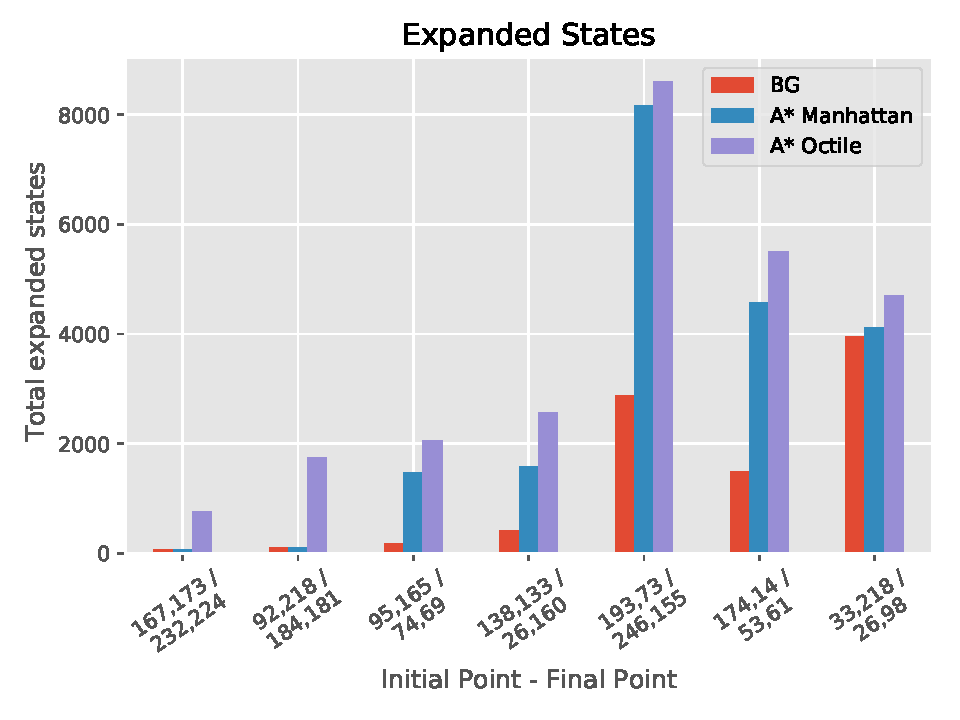
\includegraphics[width=\textwidth]{Images/Expanded_States_map1_log_heuristic.pdf}
\caption{Estados expandidos para as buscas informadas no mapa 1}
\label{fig:expanded-a1}
\end{minipage}%
\begin{minipage}{0.5\linewidth}
\centering
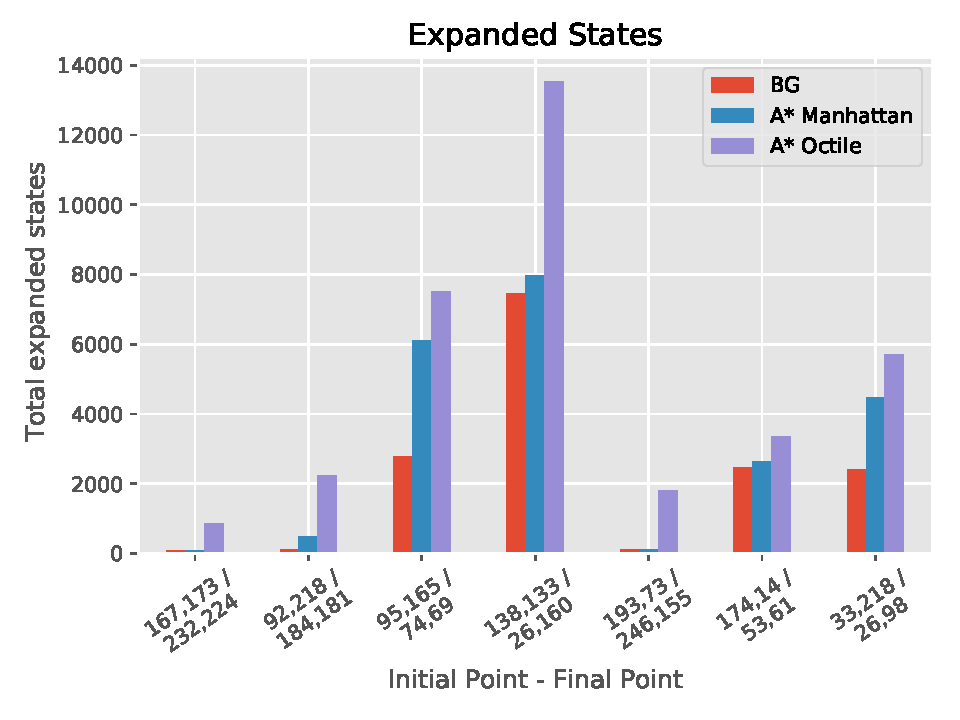
\includegraphics[width=\textwidth]{Images/Expanded_States_map2_log_heuristic.pdf}
\caption{Estados expandidos para as buscas informadas no mapa 2}
\label{fig:expanded-a2}
\end{minipage}
\begin{minipage}{0.5\linewidth}
\centering
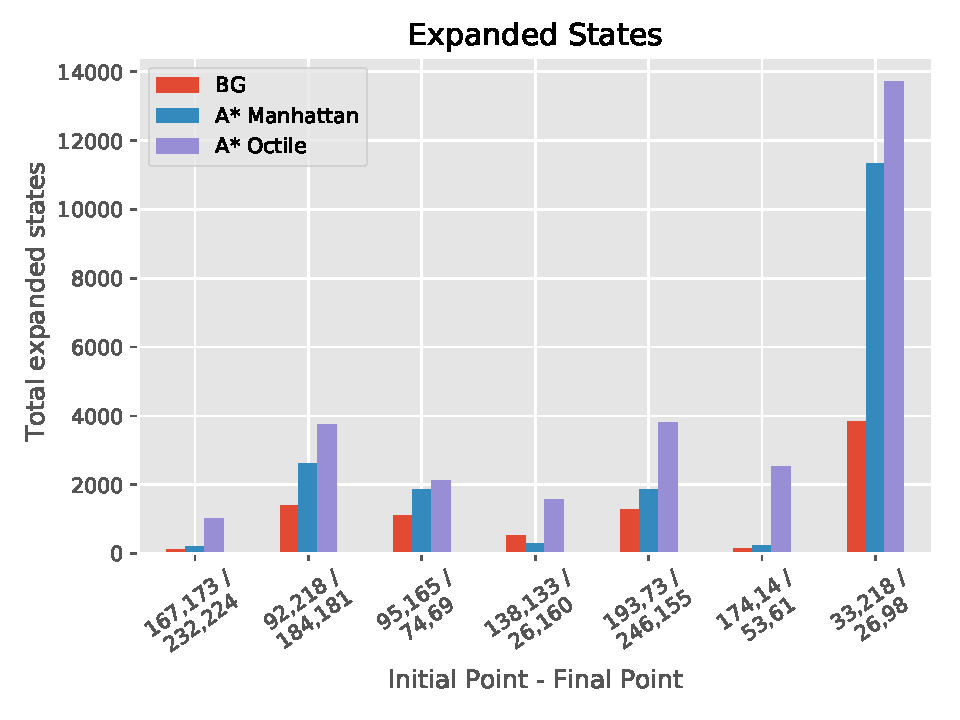
\includegraphics[width=\textwidth]{Images/Expanded_States_map3_log_heuristic.pdf}
\caption{Estados expandidos para as buscas informadas no mapa 3}
\label{fig:expanded-a3}
\end{minipage}
\end{figure}

O número de estados expandidos pelo A* com \textit{distância Manhattan} é menor do que o A* com \textit{distância octile}, como pode ser visto nas figuras~\ref{fig:expanded-a1},~\ref{fig:expanded-a2} e~\ref{fig:expanded-a3}. Dessa forma, o A* com \textit{distância Manhattan} pode não expandir estados que fazem parte do caminho ótimo. Isso é mais uma comprovação de que essa heurística não é admissível e consistente, uma vez que uma heurística consistente expande todos os estados cujo custo é menor do que o ótimo.

O número de estados expandidos por segundo é mostrado nas figuras~\ref{fig:expanded-sec1},~\ref{fig:expanded-sec2} e~\ref{fig:expanded-sec3}. É possível observar que o número de estados expandidos por segundo costuma ser maior para os algoritmos A* em relação ao UCS, em particular nos mapas 1 e 3. Isso ocorre pois esses algoritmos são mais rápidos para encontrar o resultado, expandindo os nós em um período de tempo relativamente menor. O algoritmo de UCS precisa lidar com um número maior de elementos na fronteira conforme ele expande, uma vez os nós são expandidos uniformemente em todas as direções, enquanto o A* expande de uma forma mais direcionada. Para o mapa 2, o número de nós expandidos por segundo para o UCS se mostrou maior em relação ao A* na maioria dos casos. Isso pode ter ocorrido devido a natureza do mapa, que fez com houvesse um número menor de estados para se expandir de uma vez devido a existência de caminhos mais estreitos.

\begin{figure}[!htbp]
\begin{minipage}{0.5\linewidth}
\centering
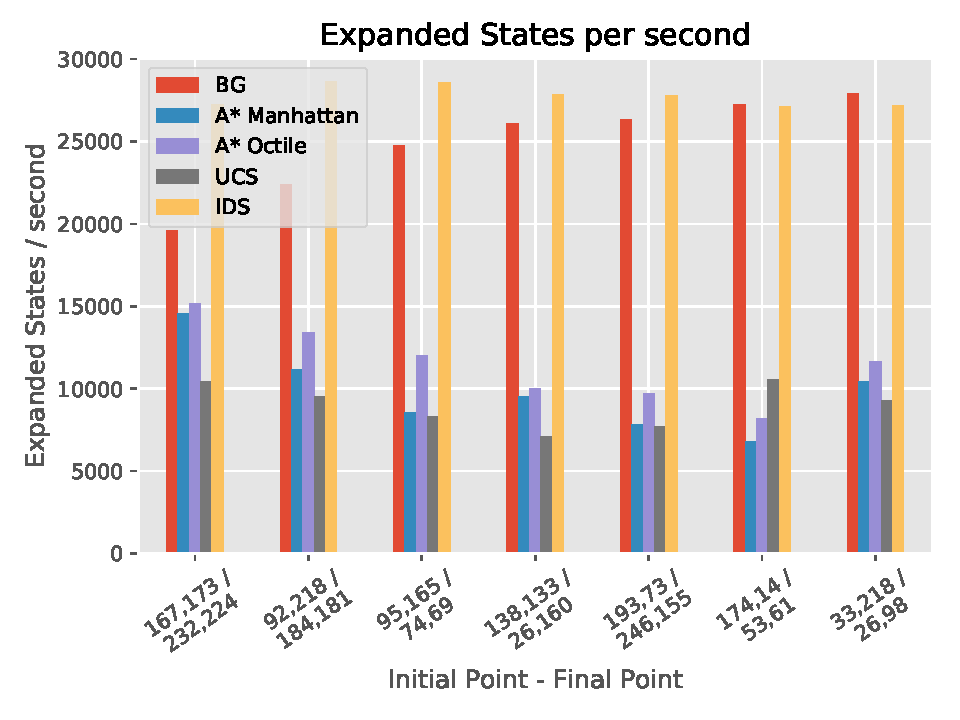
\includegraphics[width=\textwidth]{Images/Expanded_States_sec_map1.pdf}
\caption{Estados expandidos por segundo para o mapa 1}
\label{fig:expanded-sec1}
\end{minipage}%
\begin{minipage}{0.5\linewidth}
\centering
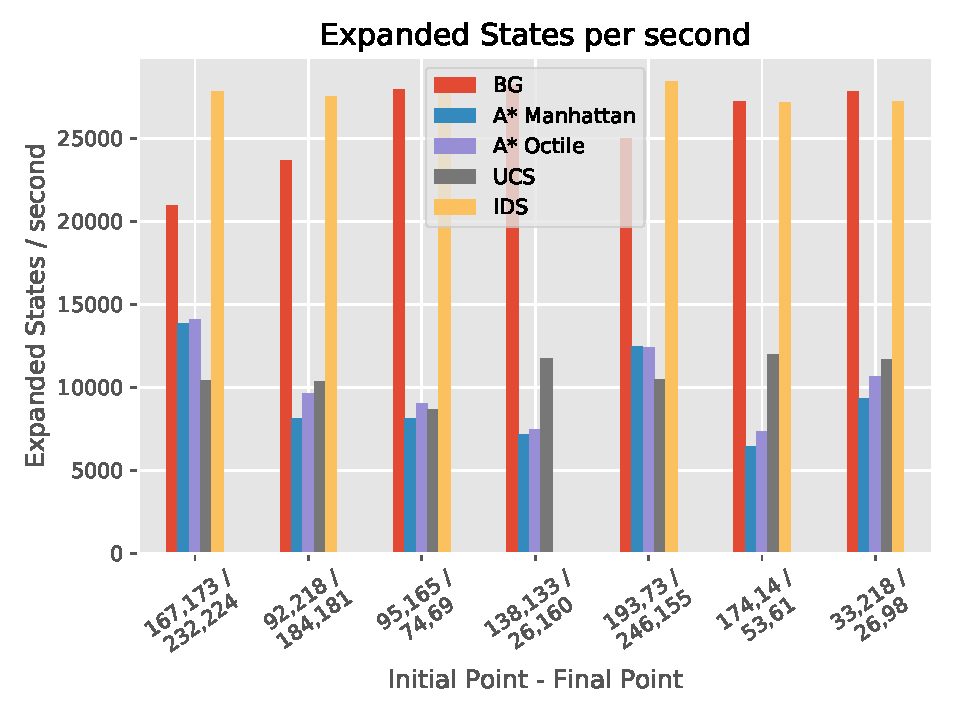
\includegraphics[width=\textwidth]{Images/Expanded_States_sec_map2.pdf}
\caption{Estados expandidos por segundo para o mapa 2}
\label{fig:expanded-sec2}
\end{minipage}
\begin{minipage}{0.5\linewidth}
\centering
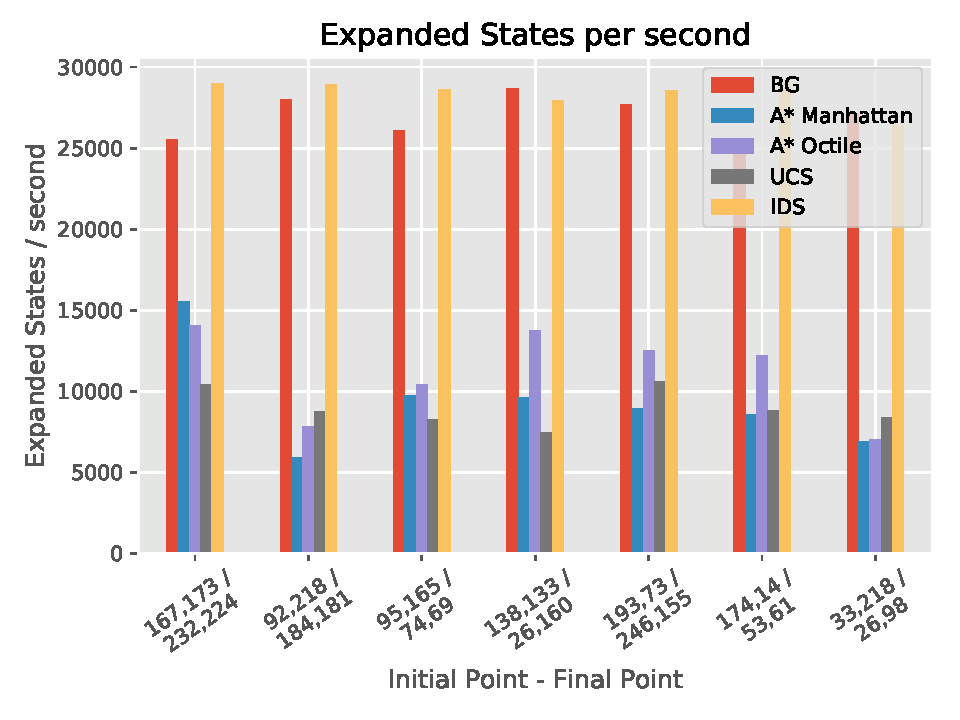
\includegraphics[width=\textwidth]{Images/Expanded_States_sec_map3.pdf}
\caption{Estados expandidos por segundo para o mapa 3}
\label{fig:expanded-sec3}
\end{minipage}
\end{figure}

\subsection{Tempo de execução}

É possível observar que o algoritmo \textit{Best first Search} é o algoritmo mais rápido dentre os examinados. Isso acontece pois ele é um algoritmo guloso, e expande o menor número de estados. O A* é o segundo mais rápido, sendo consideravelmente mais rápido que o UCS. A diferença entre essas três velocidades pode ser vista claramente nas imagens~\ref{fig:time1},~\ref{fig:time2} e~\ref{fig:time3}. O tempo do UCS, o mais lento entre os três, ainda é muito mais rápido do que o tempo do algoritmo IDS. Essas velocidades são um reflexo do número de estados expandidos por cada algoritmo.

\begin{figure}[!htbp]
\begin{minipage}{0.5\linewidth}
\centering
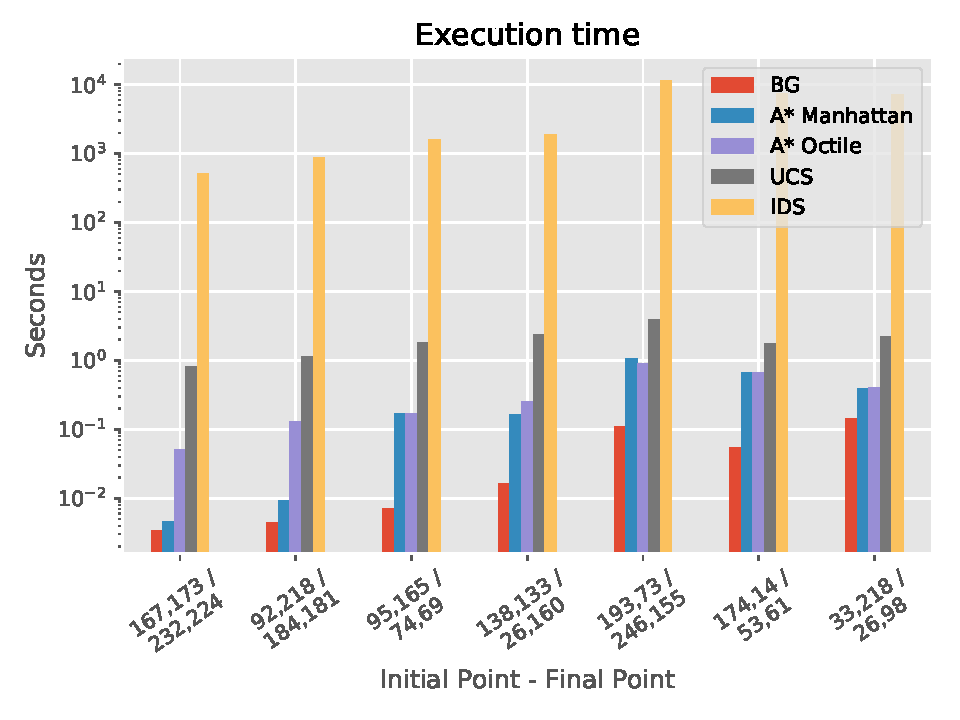
\includegraphics[width=\textwidth]{Images/Execution_time_map1_log.pdf}
\caption{Tempo de execução para o mapa 1 em escala logarítmica}
\label{fig:time1}
\end{minipage}%
\begin{minipage}{0.5\linewidth}
\centering
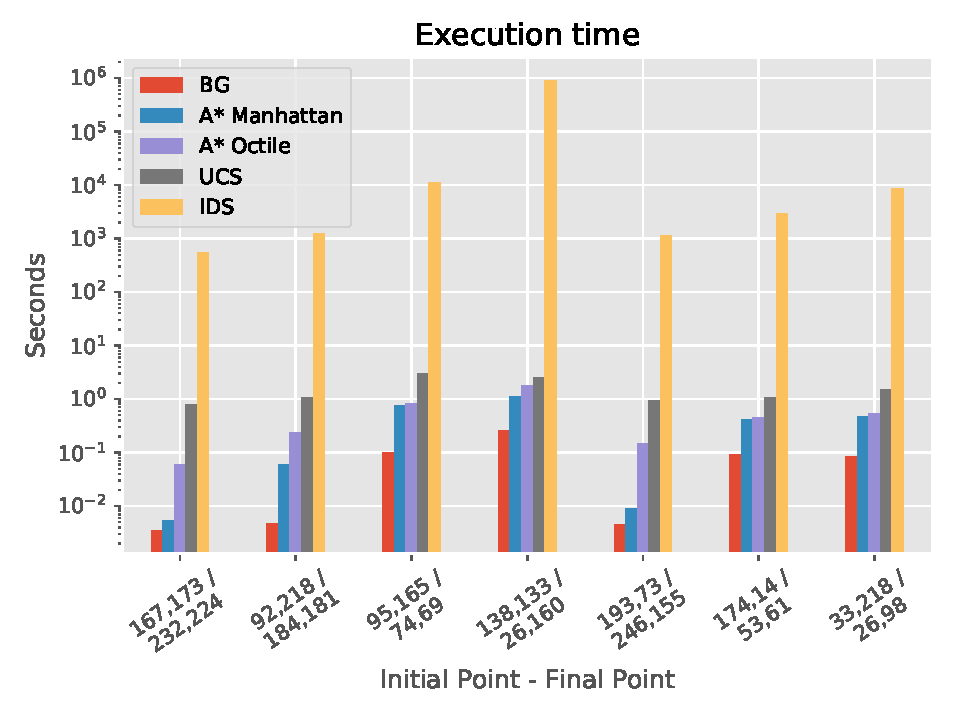
\includegraphics[width=\textwidth]{Images/Execution_time_map2_log.pdf}
\caption{Tempo de execução para o mapa 2 em escala logarítmica}
\label{fig:time2}
\end{minipage}
\begin{minipage}{0.5\linewidth}
\centering
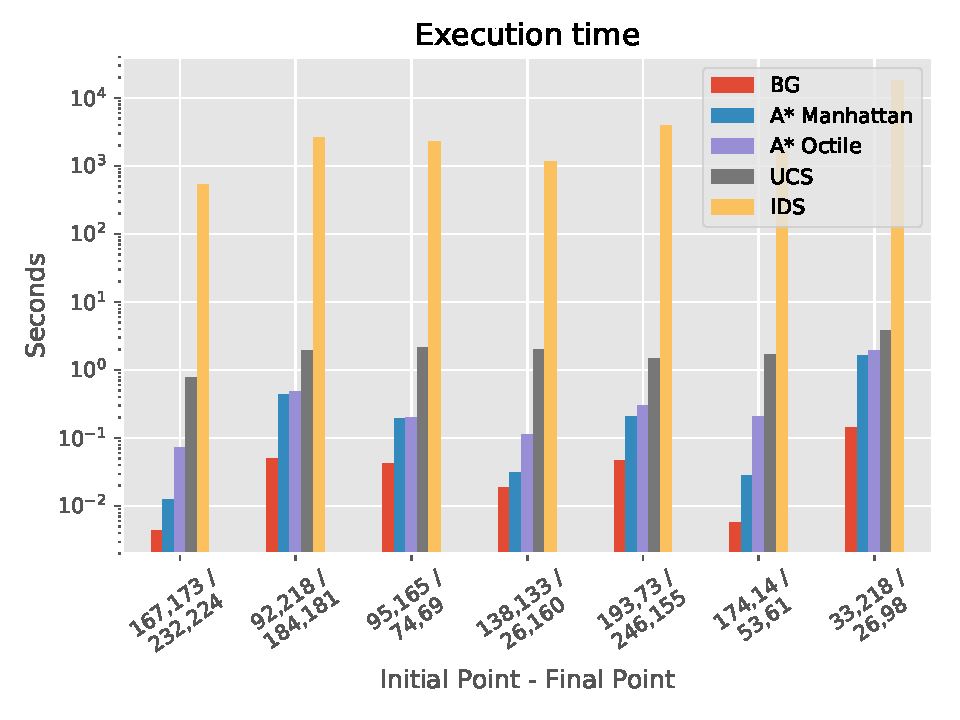
\includegraphics[width=\textwidth]{Images/Execution_time_map3_log.pdf}
\caption{Tempo de execução para o mapa 3 em escala logarítmica}
\label{fig:time3}
\end{minipage}
\end{figure}

Uma comparação melhor entre o tempo de execução dos algoritmos de busca com informação pode ser feita nas imagens~\ref{fig:time1-heur},~\ref{fig:time2-heur} e~\ref{fig:time3-heur}. O algoritmo guloso se mostra mais rápido que o A* em quase todos os exemplos testados. Isso é esperado, devido a sua característica gulosa que faz com que ele busque a primeira solução possível. O A* utilizando \textit{distância Manhattan} é mais rápido do que utilizando \textit{distância octile} na maioria das vezes, uma vez que normalmente expande menos estados.


\begin{figure}[!htb]
\begin{minipage}{0.5\linewidth}
\centering
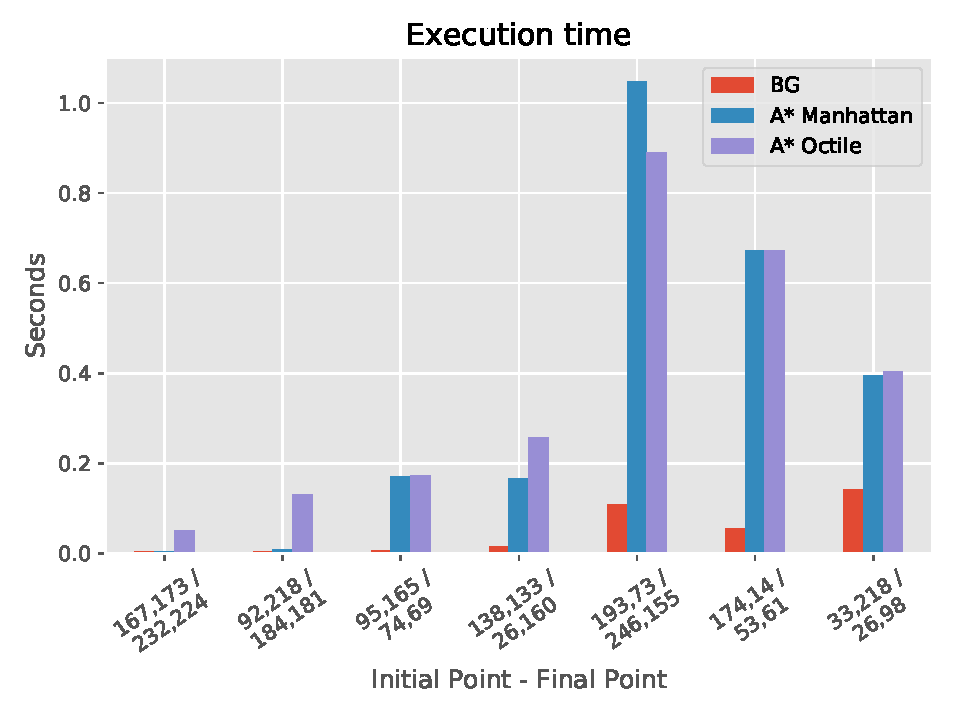
\includegraphics[width=\textwidth]{Images/Execution_time_map1_log_heuristic.pdf}
\caption{Tempo de execução para as buscas informadas no mapa 1 em escala logarítmica}
\label{fig:time1-heur}
\end{minipage}%
\begin{minipage}{0.5\linewidth}
\centering
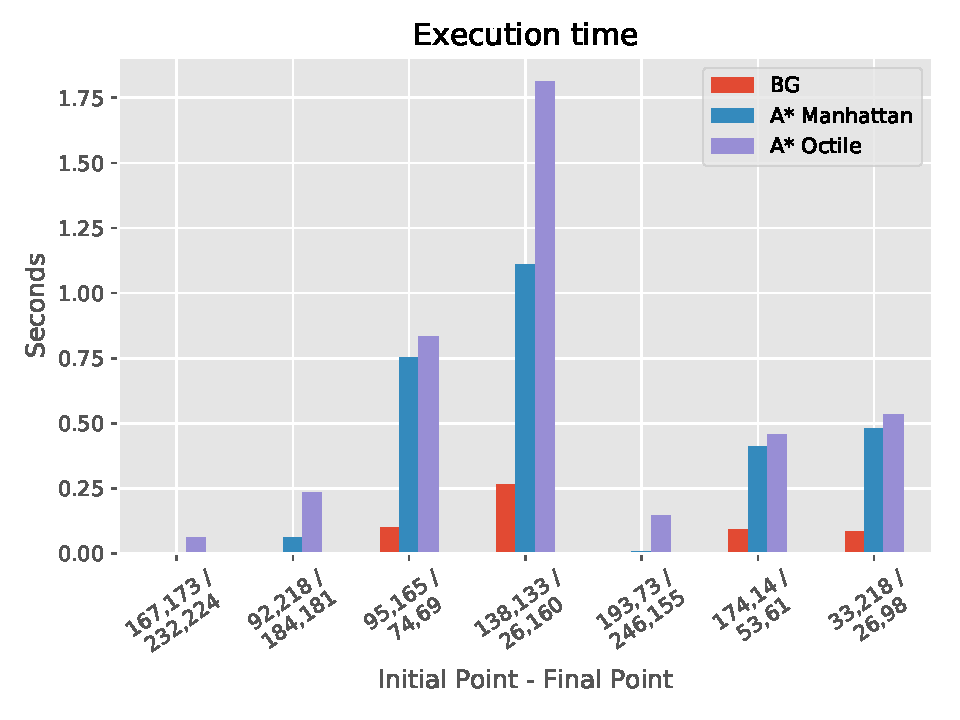
\includegraphics[width=\textwidth]{Images/Execution_time_map2_log_heuristic.pdf}
\caption{Tempo de execução para as buscas informadas no mapa 2 em escala logarítmica}
\label{fig:time2-heur}
\end{minipage}
\begin{minipage}{0.5\linewidth}
\centering
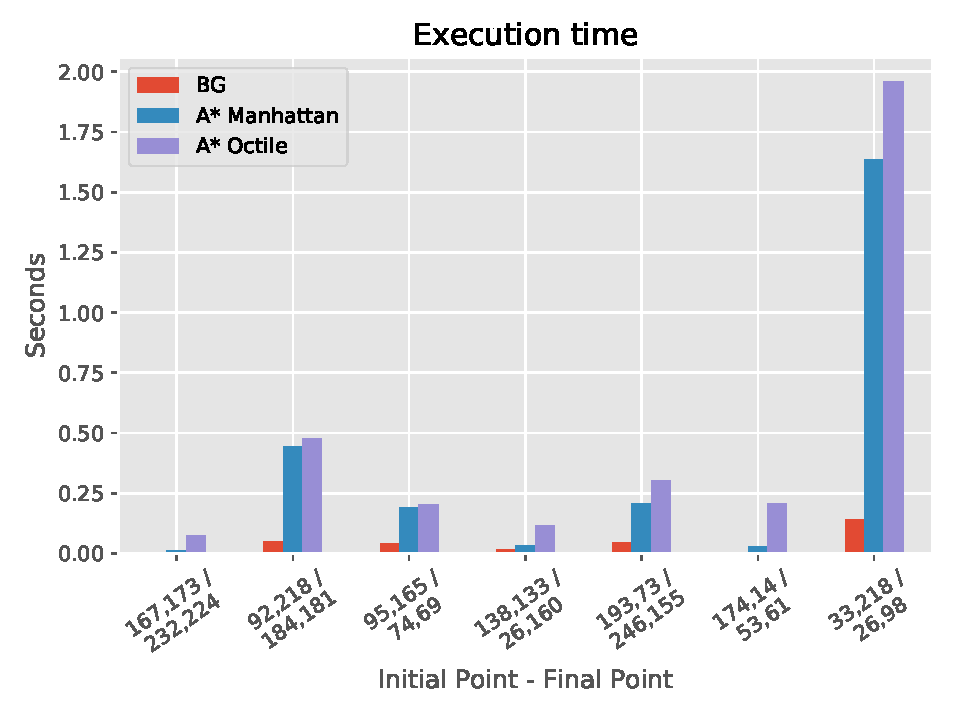
\includegraphics[width=\textwidth]{Images/Execution_time_map3_log_heuristic.pdf}
\caption{Tempo de execução para as buscas informadas no mapa 3 em escala logarítmica}
\label{fig:time3-heur}
\end{minipage}
\end{figure}